\subsection{Prinzip} 

Ein Zyklotron besteht aus 2 hohlen, halbzylindrischen Duanden, an denen eine Spannung mit unterschiedlichem Vorzeichen anliegt. Zwischen den Duanden befindet sich ein kleiner Zwischenraum, in welchem dann ein homogenes elektrisches Feld entsteht, dessen Feldlinien von der einen zur anderen Duande verlaufen (Siehe \referenz{subsec:EFeldHomogen}). Aus 2 darüber bzw. darunter liegenden Magneten ergibt sich ein homogenes Magnetfeld (Siehe \referenz{subsec:MFeldHomogen}).

Darüber hinaus gibt es einen Einlass und einen Auslass für Teilchen.\footnote{„Zyklotron Prinzipskizze02“ von KlausFoehl - Eigenes Werk. Lizenziert unter Gemeinfrei über Wikimedia Commons - \url{https://commons.wikimedia.org/wiki/File:Zyklotron_Prinzipskizze02.svg}}


\begin{wrapfigure}{o}{0.4\textwidth} \label{Zyklo}

	\vspace{-10pt}
	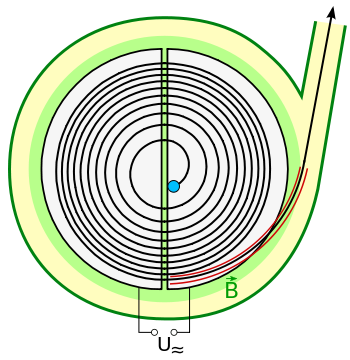
\includegraphics[width=0.35\textwidth]{Zyklotron_Prinzipskizze02.png}
	\vspace{-13pt}
	\caption{Prinzipskizze eines Zyklotrons}
	\vspace{-5pt}	
	
\end{wrapfigure}

Die Teilchenquelle im Inneren des Zyklotrons setzt Elektronen oder Protonen frei, welche durch den Einlass in das elektrische Feld zwischen den Duanden eintreten und durch dieses Feld zu einer der Beiden hin beschleunigt werden. Diese Teilchen werden gleichzeitig durch das Magnetfeld, über die Lorentzkraft, auf eine Kreisbahn gezwungen (Siehe \referenz{sec:lorentzkraft}), sodass sie im hohlen Duanden eine 180\degree{} Kurve beschreiben. Sobald wieder der Spalt zwischen den Duanden erreicht ist, wird die Spannung umgepolt, sodass die Teilchen nun zum anderen Duanden hingezogen werden. Diese Umpolungsfrequenz bleibt über den ganzen Versuch konstant.

In dem Spalt werden die Teilchen abermals und abermals beschleunigt bis der Radius so groß ist, dass die Teilchen aus dem Zyklotron austreten.


\subsection{Gesetze}

Für die Beschleunigung für \emph{Elektronen} gelten folgende Gesetzmäßigkeiten.

\subsubsection{Radius}

Aus der Gleichsetzung der Zentrifugalkraft und der Lorentzkraft ergibt sich: 

\begin{align}
\begin{split}
	F_{Zf} &= F_{Lr} \\
	\frac{m \cdot v^2}{r} &= q_e \cdot v \cdot B
\end{split}
\end{align}

\noindent Daher gilt für den Radius:

\begin{align} \label{eq:ZyklotronRadius}
\begin{split}
	r = \frac{m_e \cdot v}{B \cdot q_e}
\end{split}
\end{align}


\subsubsection{Frequenz}

Aus den Betrachtungen der Umlaufzeit $T = \frac{s_{Umlauf}}{v} = \frac{2 \pi r}{v}$ und des Radius (Siehe Gleichung \ref{eq:ZyklotronRadius}) ergibt sich für die Frequenz der Umpolung mit $f=\frac{1}{T}$: \\

\begin{align}
\begin{split}
	f &= \frac{1}{T} \\
	f &= \frac{v}{2 \pi r} \\
	f &= \frac{v \cdot q_e \cdot B}{2 \pi \cdot m_e \cdot v} \\
	f &= \frac{q_e \cdot B}{2 \pi \cdot m_e}
\end{split}
\end{align}

\noindent Damit ist gezeigt, dass die Frequenz nicht abhängig von der Geschwindigkeit der Teilchen ist und auch sonst nur von konstanten Größen abhängig ist. Daher ist die Frequenz über den gesamten Versuch konstant.




